\documentclass[twoside]{article}

\usepackage{aistats2020}
% If your paper is accepted, change the options for the package
% aistats2020 as follows:
%
%\usepackage[accepted]{aistats2020}
%
% This option will print headings for the title of your paper and
% headings for the authors names, plus a copyright note at the end of
% the first column of the first page.

% If you set papersize explicitly, activate the following three lines:
%\special{papersize = 8.5in, 11in}
%\setlength{\pdfpageheight}{11in}
%\setlength{\pdfpagewidth}{8.5in}

% If you use natbib package, activate the following three lines:
\usepackage[round]{natbib}
\renewcommand{\bibname}{References}
\renewcommand{\bibsection}{\subsubsection*{\bibname}}

% If you use BibTeX in apalike style, activate the following line:
\bibliographystyle{apalike}

% graphics
\usepackage{float}
\usepackage{graphicx}
\usepackage[usenames,dvipsnames,svgnames]{xcolor}

% math and stuff
\usepackage{amssymb}
\usepackage{amsmath}
\usepackage{amsthm}
\usepackage{bm}
\usepackage{algorithm}
\usepackage{algorithmicx}
\usepackage{algpseudocode}

% use straight double quotes in math mode
\DeclareMathSymbol{\mathdblquotechar}{\mathalpha}{letters}{`"}
\newcommand{\mathdblquote}{\mathtt{\mathdblquotechar}}
\begingroup\lccode`~=`"\lowercase{\endgroup
  \let~\mathdblquote
}
\AtBeginDocument{\mathcode`"="8000 }

% code listings
\usepackage{listings}
\lstset{
    literate={~} {$\color{black} \bm{\sim}$}{1}
}
\usepackage[framemethod=tikz]{mdframed}
%!TEX root = ./paper.tex

\lstset{
  basicstyle=\ttfamily,
  columns=fullflexible,
  keepspaces=true,
  %upquote=true,
  % Define . and % and @ as letters to include them in keywords.
  alsoletter={\.,\%,\#, \@, \?, \/, \~},
  % First type of keywords.
  % Use \bfseries\textcolor{OliveGreen} to get bolded text.
  %morekeywords=[1]{function, if, else, end, for, begin, in, const, struct, \~},
  %morekeywords=[1]{\~},
  %keywordstyle=[1]\color{red},
  % Second type of keywords.
  % Use \bfseries\textcolor{OliveGreen} to get bolded text.
   %morekeywords=[2]{\@probabilistic, \@choice},
  %keywordstyle=[2]\textcolor{Blue},
  % Add strings
  showstringspaces=False,
  %stringstyle=\ttfamily\color{NavyBlue},
  %stringstyle=\ttfamily\bfseries\color{red},
  %morestring=[b]{"},
  %morestring=[b]{'},
  morecomment=[l]{\#},
  commentstyle=\color{Gray}\ttfamily,
  moredelim=[s][\color{addresscolor}]{\{}{\}},
  %moredelim=[is][\color{distcolor}]{|}{|}
  moredelim=[is][]{|}{|}
  % l is for line comment
}

%\definecolor{codegray}{gray}{0.96}Z
\definecolor{addresscolor}{RGB}{22, 88, 12}
\definecolor{distcolor}{RGB}{40, 12, 88}
\definecolor{gencode}{RGB}{255,235,150}
%^\definecolor{jlcode}{RGB}{255, 247, 247}
\definecolor{jlcode}{RGB}{255,210,210}
%\definecolor{dslcode}{RGB}{247, 255, 230}
\definecolor{dslcode}{RGB}{220,242,255}
\usepackage{colortbl}


%\newcommand{\disc}{\mathrm{disc}}
%\newcommand{\cont}{\mathrm{cont}}
%\newcommand{\tr}{\mathtt{tr}}
%\newcommand{\model}{\mathcal{P}}
%\newcommand{\proposal}{\mathcal{Q}}
\newtheorem{theorem}{Theorem}[section]
\newtheorem{corollary}{Corollary}[theorem]
\newtheorem{lemma}[theorem]{Lemma}
\newcommand{\true}{{\mathtt{T}}}
\newcommand{\false}{{\mathtt{F}}}

\begin{document}

% If your paper is accepted and the title of your paper is very long,
% the style will print as headings an error message. Use the following
% command to supply a shorter title of your paper so that it can be
% used as headings.
%
%\runningtitle{I use this title instead because the last one was very long}

% If your paper is accepted and the number of authors is large, the
% style will print as headings an error message. Use the following
% command to supply a shorter version of the authors names so that
% they can be used as headings (for example, use only the surnames)
%
%\runningauthor{Surname 1, Surname 2, Surname 3, ...., Surname n}

\twocolumn[

\aistatstitle{Automated Involutive MCMC}

\aistatsauthor{ Marco Cusumano-Towner \And Alexander K. Lew \And Vikash K. Mansinghka }

\aistatsaddress{ Massachusetts Institute of Technology } ]

\begin{abstract}
Involutive MCMC is a unifying framework for MCMC that encompasses many standard
and recent MCMC algorithms from the literature, from reversible jump MCMC to
Hamiltonian Monte Carlo to kernels based on deep neural networks. The key idea
in involutive MCMC is that a combination of (i) an auxiliary probability
distribution and (ii) an involution on the extended state space that includes
the model latent variables and the auxiliary variables results in MCMC kernels
that satisfy detailed balance with respect to the target distribution. The
involutive MCMC framework is appealing for its simplicity and generality, and
promises to be a useful conceptual and mathematical tool for exploring the
design space of MCMC kernels. However, like other Monte Carlo samplers,
implementing involutive samplers is time consuming and error prone. This paper
describes a technique for automatically generating the implementation of
involutive MCMC samplers from two probabilistic programs that define the target
distribution and the auxiliary probability distribution respectively, and a
differentiable program that defines the involution. The technique also detects
common conceptual and programming errors that arise when designing and
specifying involutive MCMC algorithms. This paper describes the support for
involutive MCMC in the Gen probabilistic system that uses this technique, and
shows involutive samplers specified using Gen's high-level probabilistic and
differentiable programming languages.
\end{abstract}

\section{INTRODUCTION}

%This is the best paper~\citep{cusumano2019gen}.

\subsection{Second Level Heading}

\subsubsection{Third Level Heading}

\paragraph{Fourth Level Heading}

\section{BACKGROUND AND RELATED WORK}

%\subsection{Traces}

\begin{figure*}[ht]
    \centering
    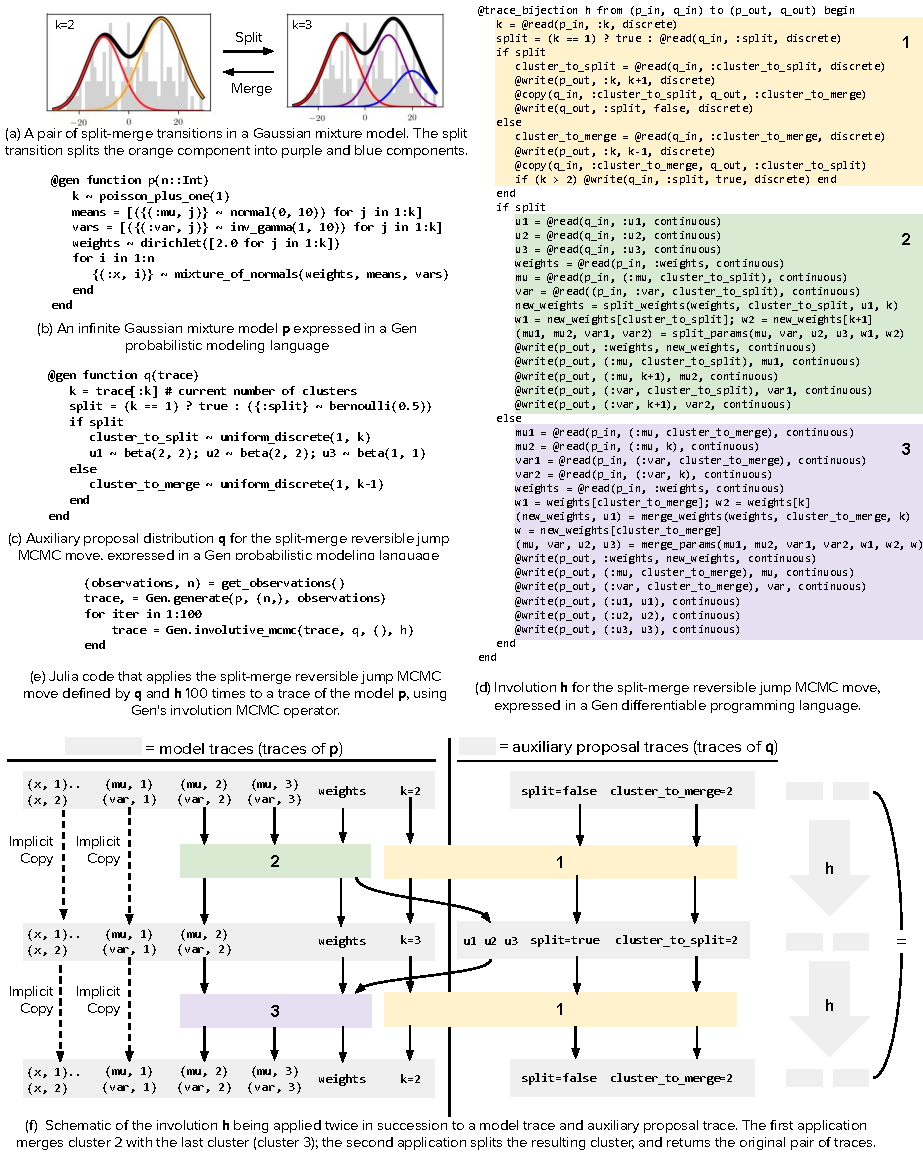
\includegraphics[width=\textwidth]{figures/mixture.pdf}
    \caption{
Example of reversible jump MCMC~\citep{green1995reversible} implemented using involutive MCMC in Gen.
The example implements a `split-merge move' in a infinite Gaussian mixture model~\citep{richardson1997bayesian} using three Gen programs:
(1) a probabilistic program $\mathtt{p}$ encoding the generative model (shown in b),
(2) a probabilistic program $\mathtt{q}$ encoding an auxiliary probability distribution (shown in c),
and (3) a differentiable program $\mathtt{h}$ that encodes an involution on the space of pairs of traces of $\mathtt{p}$ and $\mathtt{q}$ (shown in d).
Gen's involutive MCMC operator (shown in e) automatically computes the acceptance probability.
}
    \label{fig:mixture}
\end{figure*}

\begin{figure*}[ht]
    \centering
    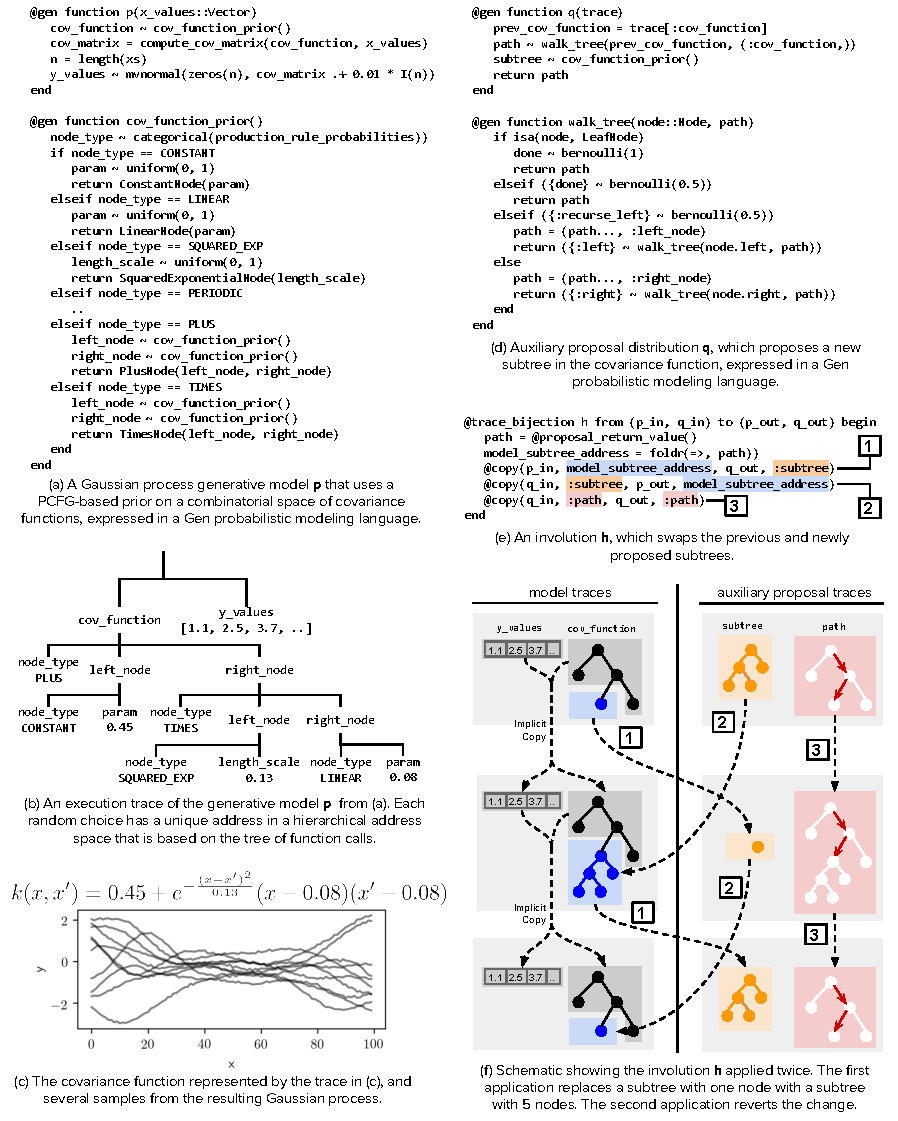
\includegraphics[width=\textwidth]{figures/structure-learning.pdf}
    \caption{
A mixture kernel implemented using involutive MCMC in Gen, applied to infer the covariance function of a Gaussian process.
The prior on covariance functions is based on a probabilistic context-free grammar.
Each component kernel in the mixture replaces a subtree of the covariance function parse tree with a new subtree.
The mixture kernel chooses a random subtree to replace via a random walk on the parse tree.
The mixture kernel is composed from three Gen programs:
(1) a probabilistic program $\mathtt{p}$ encoding the generative model (shown in a),
(2) a probabilistic program $\mathtt{q}$ encoding an auxiliary probability distribution (shown in b), and
(3) a differentiable program $\mathtt{h}$ that encodes an involution (shown in d).
}
    \label{fig:structure-learning}
\end{figure*}

\section{INVOLUTIVE MCMC} \label{sec:involutive-mcmc}
Let $(X, \Sigma_P, \mu_P)$ and $(Y, \Sigma_Q, \mu_Q)$ denote two measure spaces with $\sigma$-finite $\mu_P$ and $\mu_Q$.
Let $p : X \to [0, \infty)$ be a probability density with respect to $\mu_P$ and for each $x \in X$ such that $p(x) > 0$ let $q_x : Y \to [0, \infty)$ be probability density with respect to $\mu_Q$.
We call $p$ the \emph{model density} and we call $q_x$ \emph{auxiliary densities}.
Let $\pi(x, y) := p(x) q_x(y)$ and $Z := \{(x, y) \in X \times Y : \pi(x, y) > 0 \}$.
Suppose that $Z \in \Sigma_P \otimes \Sigma_Q$ ($Z$ is a $\mu_P \times \mu_Q$-measurable set).
Then $\Sigma := \{A \in \Sigma_P \otimes \Sigma_Q : A \subseteq Z\}$ is a $\sigma$-algebra on $Z$ and $\mu : \Sigma \to [0, \infty)$ with $\mu(A) := (\mu_P \times \mu_Q)(A)$ is a $\sigma$-finite measure on measurable space $(Z, \Sigma)$.

Let $f : Z \to Z$ denote an involution ($f^{-1} = f$) such that the pushforward of $\mu$ under $f$, denoted $\mu \circ f^{-1}$, is absolutely continuous with respect to $\mu$, with Radon-Nikodym derivative $d (\mu \circ f^{-1}) / d\mu : Z \to [0, \infty)$.
Let $y \sim q_x(\cdot)$ denote a random sample from the measure defined by $A \mapsto \int_A q_x(y) \mu_Q(dy)$ for $A \in \Sigma_Q$.

\begin{algorithm}[h]
\begin{algorithmic}
\Procedure{involutive-mcmc-move}{$p$, $q$, $f$, $x$}
    \State $y \sim q_x(\cdot)$ \Comment{Sample auxiliary variables}
    \State $(x', y') \gets f(x, y)$ \Comment{Apply involution}
    \State $\alpha \gets
        \displaystyle \frac{p(x') q_{x'}(y')}{p(x) q_{x}(y)} \left( \frac{d (\mu \circ f^{-1})}{d \mu} (x, y)\right)$
    % TODO check it
    \State $r \sim \mathrm{Uniform}(0, 1)$
    \State \algorithmicif \, $r \le \alpha$ \algorithmicthen \, \Return $x'$ \algorithmicelse \, \Return $x$ 
\EndProcedure
\end{algorithmic}
\caption{Involutive MCMC}
\label{alg:involutive-mcmc}
\end{algorithm}

See Section~\ref{sec:radon-nikodym-special-case} for a derivation of the Radon-Nikodym derivative $d (\mu \circ f^{-1}) / d \mu$ for a special case, when the involution $f$ can be factored into (i) an involution on a countable partition of $Z$ and (ii) a family of continuously differentiable bijection on Euclidean spaces.

\begin{theorem}[Involutive MCMC is stationary]
Algorithm~\ref{alg:involutive-mcmc} defines a probability kernel $k$ on $X$ that is stationary with respect to the model probability distribution.
That is, $\int_X k_x(B) p(x) d\mu_X(dx) = \int_B p(x) d\mu_X(dx)$ for all $B \in \Sigma_X$.
\end{theorem}
\begin{proof}
The proof is presented in stages in the appendix (see Section~\ref{sec:involution-detailed-balance}, Section~\ref{sec:involution-is-stationary}, and Section~\ref{sec:involutive-mcmc-is-stationary}).
\end{proof}

\section{PROBABILISTIC PROGRAMMING WITH TRACES}

Probabilistic programs are programs that define probability distributions.
Probabilistic programs can be used to define standard joint probability distributions over vectors of random-variables, as well as more complex probability distributions with uncertainty over the structure in which the set of random variables itself random.
Involutive MCMC can be applied for target probability distributions on non-standard reference measures, including models with structure uncertainty.
For example, reversible jump MCMC, which is a special case of involutive MCMC, can be applied to switch between different model structures.
This section describes a framework for probabilistic programming that is expressive enough to represent probability distributions with structure uncertainty.

In our framework, a probabilistic program defines a probability distribution on finite dictionaries that map the identifer for a random choice (called its \emph{address}) to its value.
Following standard terminology~\citep{?}, we call these dictionaries \emph{traces} because they are often sampled by running a probabilistic program, and `tracing' the execution the program by recording the value of eacn random choice encountered.
The next section makes the concept of a trace more concrete using code in a probabilistic programming language.

\subsection{A Probabilistic Programming Language}

The probabilistic programming language used in this paper is based on the dynamic modeling language in the Gen probabilistic programming system~\citep{gen-pldi}.
In this language, user tags each random choice with an explicit address in the code, as part of a \emph{random-choice expression} of the following form:
\noindent
\begin{center}
\begin{tabular}{c}
{\begin{lstlisting}[basicstyle=\small\ttfamily]
{<address>} ~ <distribution>
\end{lstlisting}}
\end{tabular}
\end{center}
The left-hand side of the expression (green) specifies the address of the choice, and the right-hand side specifies the probability distribution to be sampled from.
For example, the following expression samples a non-negative integer from a geometric distribution and the value gets recorded in the trace at the address \texttt{"a"}:
\noindent
\begin{center}
\begin{tabular}{c}
{\begin{lstlisting}[basicstyle=\small\ttfamily]
{"a"} ~ geometric(0.5)
\end{lstlisting}}
\end{tabular}
\end{center}
In addition to being recorded in the trace, the sampled value is returned to the running program.
That is, the random choice expression evaluates to the sampled value.
For example, the expression below evaluates to a an even non-negative integer:
\noindent
\begin{center}
\begin{tabular}{c}
{\begin{lstlisting}[basicstyle=\small\ttfamily]
({"a"} ~ geometric(0.5)) * 2
\end{lstlisting}}
\end{tabular}
\end{center}
Probabilistic programs are typically constructed by combining multiple random choice expressions with regular Julia code (Gen is embedded in the Julia programming language~\citep{julia}).
\noindent
\begin{center}
\begin{tabular}{c}
{\begin{lstlisting}[basicstyle=\small\ttfamily]
a = ({"a"} ~ geometric(0.5))
{"b"} ~ bernoulli(a / (a + 1))
\end{lstlisting}}
\end{tabular}
\end{center}
This probabilistic program has an unbounded (countably infinite) number of possible traces it could produce.
One possible trace samples the value 1 at $\texttt{"a"}$ and the Boolean value $\false$ at \texttt{"b"}, and we denote this trace by $\{\mathtt{"a"} \mapsto 1, \mathtt{"b"} \mapsto \false\}$.
Note that the variable to which the first choice was assigned happens to be the same as the address.
This is not required, and often the random choice has no variable name in the program, as in the second random choice with address \texttt{"b"}.
But to reduce possibe unecessary typing, the following optional syntactic sugar will simultaneously assign the value to the program variable $\mathtt{a}$ and record it at trace address $\mathtt{a}$.\footnote{
More precisely, the address is the Julia symbol (interned string) \texttt{a}, constructed with Julia syntax \texttt{:a}.}
\noindent
\begin{center}
\begin{tabular}{c}
{\begin{lstlisting}[basicstyle=\small\ttfamily]
a ~ geometric(0.5)
\end{lstlisting}}
\end{tabular}
\end{center}
Probabilistic programs can make use of familiar control flow constructs, like loops and branching.
Stochastic control flow is also possible:
\noindent
\begin{center}
\begin{tabular}{c}
{\begin{lstlisting}[basicstyle=\small\ttfamily]
i = 1
while ({i} ~ bernoulli(0.5))
    i = i + 1
end
\end{lstlisting}}
\end{tabular}
\end{center}
Note that for the probabilistic program to be valid, we require that every address is used at most once within every possible execution.

For probabilistic programs that sample from discrete probability distributions like those used above, the meaning of the program is a probability mass function $p$ that assigns a probability to every possible trace.
For example, for the program with the \texttt{while} loop above, the distribution is:
\[
\begin{array}{c|c}
    x & p(x)\\
    \hline
    \{1 \mapsto \false\} & 0.5\\
    \{1 \mapsto \true, 2 \mapsto \false\} & 0.5^2\\
    \{1 \mapsto \true, 2 \mapsto \true, 3 \mapsto \false\} & 0.5^3\\
    .. & ..
\end{array}
\]
We assume that probabilistic programs halt with probability $1$, meaning that the sum of probabilities over all (finite) traces is one.
Note that traces are always finite, but there may be an infinite number of possible traces, as in the previous example.

In order to construct more complex distributions, we wrap probabilistic programs in functions, called
`generative functions' in Gen.
These functions can then be invoked by other functions, including recursively, which allows programs encode probability distributions on more complex and combinatorial objects.
When invoking such a function, we give an \emph{address namespace} under which every random choice made in that function should be recorded.
This helps prevent addresses of choices defined in different functions from colliding.
The syntax for calling a generative function and assigning the address namespace is the same as that of random choice expressions.
For example:
\begin{center}
\begin{tabular}{c}
\begin{lstlisting}[basicstyle=\small\ttfamily]
@gen function g()
  if ({"go"} ~ bernoulli(0.2))
    n1 = ({"L"} ~ g())
    n2 = ({"R"} ~ g())
    return n1 + n2 + 1
  else
    return 1
  end
end
\end{lstlisting}
\end{tabular}
\end{center}
Because this is a recursive function, a the trace is populated with a hierarchy of addresses.
For example, the first random choice in the first recursive call has address \texttt{"L"."go"}.
When this function is invoked it encodes the following probability distribution on traces (quotation marks omitted from addresses to improve readability):
\[
\begin{array}{c|c}
    x & p(x)\\
    \hline
    \left\{\mathtt{go} \mapsto \false\right\} & 0.8\\
& \\
    \left\{\begin{array}{c}
        \mathtt{go} \mapsto \true, \mathtt{L}.\mathtt{go} \mapsto \false, \mathtt{R}.\mathtt{go} \mapsto \false
    \end{array}\right\} & 0.2 \cdot 0.8^2\\
& \\
    \left\{\begin{array}{c}
        \mathtt{go} \mapsto \true,
        \mathtt{L}.\mathtt{go} \mapsto \true,
        \mathtt{R}.\mathtt{go} \mapsto \false,\\
        \mathtt{L}.\mathtt{L}.\mathtt{go} \mapsto \false,
        \mathtt{L}.\mathtt{R}.\mathtt{go} \mapsto \false
    \end{array}\right\}& 0.2^2 \cdot 0.8^3\\
     .. & ..
\end{array}
\]


% measure version
\subsection{Handling Continuous Distributions}
For programs that can sample from continuous probability distributions, the formalism needs to be extended.
Let $\mathcal{A}$ denote a set of addresses.
For each address $a \in \mathcal{A}$ we assign a reference measure space $(V_a, \Sigma_a, \mu_a)$ where $\mu_a$ is $\sigma$-finite ($V$ stands for `values').
Let $T := \cup_{A \subseteq \mathcal{A} : |A| < \infty} \{(A, \mathbf{x}) : \mathbf{x} \in \times_{a \in A} V_a\}\}$ denote the set of all finite traces (i.e. dictionaries) from addresses in $\mathcal{A}$ to their values.
For each finite $A \subseteq \mathcal{A}$, let $\Sigma_A := \otimes_{a \in A} \Sigma_a$ (the product $\sigma$-algebra over $\Sigma_a$ for $a \in A$), and let $\mu_A := \times_{a \in A} \mu_a$ (the product measure).
Let $\Sigma \subseteq \mathcal{P}(T)$ be the $\sigma$-algebra formed by sets of the form $B := \cup_{A \subseteq \mathcal{A}, |A| < \infty} \{(A, \mathbf{x}) : \mathbf{x} \in B_A\}$ for some $B_A \in \Sigma_A$ for each $A$.
Let $\mu : \Sigma \to [0, \infty)$ be a measure on measurable space $(T, \Sigma)$ defined by $\mu(B) := \sum_{A \subseteq \mathcal{A}, |A| < \infty} \mu_A(B_A)$.

A probabilistic program $P$ denotes a probability density $p : T \to [0, \infty)$ with respect to a reference measure $\mu$ on traces.
Describing the denotational semantics of a particular probabilistic programming language (the function mapping programs $P$ to density functions $p$) is out of scope for this paper.
We refer to the reader to~\citet{popl} for an example of denotational semantics of a probabilistic programming language that uses explicit addresses for random-choices.

This formalism is capable of expressing probabilistic programs that use continuous distributions by setting the reference measure space $(V_a, \Sigma_a, \mu_a)$ for some addresses $a$ to use the Lebesgue-measure.
For example, consider the following probabilistic program:

TODO: Give an example of a probabilistic program in Gen's dynamic modeling language that includes continuous random choices, and show the reference measure on traces and its density.
\noindent
\begin{center}
\begin{tabular}{c}
{\begin{lstlisting}[basicstyle=\small\ttfamily]
@gen function foo(x1, x2, x3)
  a = ({:a} ~ bernoulli(x1))
  b = ({:b} ~ bernoulli(x2))
  c = ({:c} ~ bernoulli(x3))
  {:d} ~ bernoulli((a && b && c) ? 0.9 : 0.1)
  return a && b && c && d
end
\end{lstlisting}}
\end{tabular}
\end{center}


TODO: somewhere, talk about hierarchical addresses
%\paragraph{Hierarchical addresses}

\subsection{Involutive MCMC with probabilistic programs}

To define the model and auxiliary densitites used in involutive MCMC in Section~\ref{sec:involutive-mcmc} using probabilistic programs, we write one probabilistic program ($P$) to define the model's probability distribution, and another probabilistic program ($Q$) to define the set of auxiliary distributions.
The model reference measure $(X, \Sigma_P, \mu_P)$ and density that were required in Section~\ref{sec:involutive-mcmc} are set to the probabilistic program's reference measure and density $p$ on traces as defined above (so that $X := T$).
To define the auxiliary densities, we use a second probabilistic program $Q$ that is parametrized by (i.e. takes as input) traces of the model program $P$.
The set of possible inputs to $Q$ is $\{x \in T : p(x) > 0\}$, and for each such $x$ the probabilistic program $Q$ defines a density $q_x : T \to [0, \infty)$ with respect to the reference measure on traces.\footnote{
Note that we the same measure space $(T, \Sigma, \mu)$ on traces for both the model and auxiliary probabilistic program.
If both programs sample some random choice at the same address $a$ and require different measure spaces $(V_a, \Sigma_a, \mu_a)$ for the address, this can be handled formally by making the addresses sampled by the two programs disjoint by prepending either the prefix `p.' or `q.' to addresses.
This is only required for book-keeping in the formalism, and these prefixes do not need to be actually added to the addresses used in the programs.}

The involutive MCMC framework of Section~\ref{sec:involutive-mcmc} requires that $Z := \{(x, y) \in X \times Y : \pi(x, y) > 0\}$ is $\mu_P \times \mu_Q$-measurable.
We now give a sufficient condition for this to hold.
Let $D \subseteq \mathcal{A}$ denote the subset of addresses that are discrete (i.e. where $V_a$ is a countable set and $\mu_a$ is the counting measure).
For $\mathbf{x} \in \times_{a \in A} V_a$ let $\mathbf{x} = (\mathbf{d}, \mathbf{c})$ where $\mathbf{d} \in \times_{a \in A \cap D} V_a$ and $\mathbf{c} = \times_{a \in A \setminus D} V_a$, so that $\mathbf{d}$ is the discrete part of $\mathbf{x}$ and $\mathbf{c}$ is the non-discrete part.
 %TODO make this a proposition
\begin{lemma}
Suppose that $p$ and $q$ are such that $p(A, (\mathbf{d}, \mathbf{c})) > 0$ implies
$p(A, (\mathbf{d}, \mathbf{c}')) > 0$ for all $\mathbf{c}' \in \prod_{a \in A \setminus D} V_a$,
and that $q_x(A, (\mathbf{d}, \mathbf{c})) > 0$ where $x = (\tilde{A}, \tilde{\mathbf{d}}, \tilde{\mathbf{c}})$ implies that
$q_{x'}(A, (\mathbf{d}, \mathbf{c}')) > 0$ for all $\mathbf{c}' \in \prod_{a \in A \setminus D} V_a$ and all $x' = (\tilde{A}, \tilde{\mathbf{d}}, \tilde{\mathbf{c}}')$ where $\tilde{\mathbf{c}}' \in \prod_{a \in \tilde{A} \setminus D} V_a$.
Then, $Z := \{(x, y) \in X \times Y : \pi(x, y) > 0\}$ is $\mu \times \mu$-measurable where $\mu$ is the reference measure on traces.
\end{lemma}
\begin{proof}
For $p$ and $q$ satisfying these conditions,
$Z = \cup_{(A_1,A_2,\mathbf{d}_1,\mathbf{d}_2) \in E} \{((A_1, (\mathbf{d}_1, \mathbf{c}_1)), (A_2, (\mathbf{d}_2, \mathbf{c}_2))) : \mathbf{c}_1 \in \times_{a \in A_1 \setminus D} V_a, \mathbf{c}_2 \in \times_{a \in A_2 \setminus D} V_a\}$ for some countable set $E \subseteq \{(A_1, A_2, \mathbf{d}_1, \mathbf{d}_2) : A_1, A_2 \subseteq \mathcal{A}, |A_1| < \infty, |A_2| < \infty, \mathbf{d}_1 \in \times_{a \in A_1 \cap D} V_a, \mathbf{d}_2 \in \times_{a \in A_2 \cap D} V_a\}$ of address sets and discrete choice values for both programs.
The measure of $Z$ is
$(\mu \times \mu)(Z) = \sum_{(A_1,A_2,\mathbf{d}_1,\mathbf{d}_2) \in E} \prod_{a \in (A_1 \setminus D) \cup (A_2 \setminus D)} \mu_a(V_a)$.
% TODO double check me.,
\end{proof}

Intuitively, this requirement means that for both the model probabilistic program $P$ and the auxiliary probabilistic program $Q$, the support of a random choice that is not discrete cannot depend on the value of another non-discrete random choice.
Additionally, the support of non-discrete random choices in $Q$ cannot depend on the value of non-discrete random choices in the input $x$, which is a trace of $P$.

%\paragraph{Conditioning}

\section{DIFFERENTIABLE PROGRAMMING WITH TRACES}

% TODO PyTorch implementation??

\section{AUTOMATIC ACCEPTANCE PROBABILITY CALCULATION}


% TODO can only show this for a special case -- discrete involution + continuous?, or some more general case?

% TODO show an performance table of moves per second with and without the sparsity reduction (?)

\section{A DYNAMIC CHECK FOR DETECTING BUGS}

% TODO show an example of the type of bug it can detect (an edge case?)

\section{EXAMPLES}


\subsubsection*{Acknowledgements}
All acknowledgments go at the end of the paper, including thanks to reviewers who gave useful comments, to colleagues who contributed to the ideas, and to funding agencies and corporate sponsors that provided financial support.

\bibliography{references} 

\clearpage
\onecolumn
\section*{APPENDIX}

%\subsection{Distributions on traces}
%% TODO rewrite this section..
%Define target density $\pi$ (XXX below it is called $p$, fix this) on the joint space $X \times U$, where $X$ are traces of the model and $X$ are traces of the proposal, in terms of the density $p(x)$ and the family of densities $q_x(u)$ as $\pi(x, u) := p(x) q_u(x)$.
%
%% TODO rename the joint target density to \pi below
%We want to show stationarity with respect to $\pi$, using stationarity of the involution with respect to the joint density (below).
%\begin{equation}
%\int_X p(x) \ell_x(A) \mu(dx) = p(A) \mbox{ for all } A \in \Sigma
%\end{equation}
%where $\ell_x(A)$ is the probability of transitioning into set $A$ from $x$, and is given by:
%\begin{equation}
%\ell_x(A) := \int_U k_{(x, u)}(A \times U) \mu(du)
%\end{equation}
%where $k_{(x, u)}$ is the measure on $X \times U$ that is induced by applying the involution $h$ to the state $(x, u)$.
% TODO checkme


\subsection{Derivation of the pushforward Radon-Nikodym derivative for a special case} \label{sec:radon-nikodym-special-case}
Implementing Algorithm~\ref{alg:involutive-mcmc} requires computing the Radon-Nikodym derivative $d (\mu \circ f^{-1}) / d \mu$.
This section derives that function for the special case in which the involution $f$ can be factored into an involution on a countable set $I$ and a family of bijections on $\mathbb{R}^{n_i}$ for some $n_i$ for each $i \in I$.
Suppose $Z = \{(i, \mathbf{x}) : i \in I, \mathbf{x} \in \mathbb{R}^{n_i}\}$.
Suppose $f_1$ is an involution on $I$ and $n_i = n_{f_1(i)}$ and $f_2$ is a family of continuously differentiable bijections indexed by $i \in I$, such that $f_{2,i} : \mathbb{R}^{n_i} \to \mathbb{R}^{n_i}$.
Also suppose that $f_{2,i} = f_{2,f_1(i)}^{-1}$ for all $i \in I$. That is,
\begin{equation}
f_{2,i}(f_{2,f_1(i)}(\mathbf{x})) = \mathbf{x} \mbox{ for all } \mathbf{x} \in \mathbb{R}^{n_i} \mbox{ and all } i \in I
\end{equation} 
Then, $f : Z \to Z : (i, \mathbf{x}) \mapsto (f_1(i), f_{2,i}(\mathbf{x}))$ is an involution because:
\begin{equation}
f(f(i, \mathbf{x})) = f(f_1(i), f_{2,i}(\mathbf{x})) = (f_1(f_1(i)), f_{2,f_1(i)}(f_{2,i}(\mathbf{x}))) = (i, \mathbf{x})
\end{equation}
Let $\Sigma_n$ and $\mu_n$ denote the Lebesgue $\sigma$-algebra and Lebesgue measure on $\mathbb{R}^n$, respectively.
Let $\Sigma \subset \mathcal{P}(Z)$ be the $\sigma$-algebra of sets of the form $\cup_{i \in I} \{(i, \mathbf{x}) : \mathbf{x} \in A_i\}$ for some $A_i \in \Sigma_{n_i}$ for each $i \in I$.
%Let $\Sigma$ be the $\sigma$-algebra on $Z$ generated by the sets $G := \{ \{(i, \mathbf{x}) : \mathbf{x} \in A\} : i \in I, A \in \Sigma_{n_i} \}$.
%Note that the sets $G$ form a $\pi$-system:
%\begin{align}
%\{(i, \mathbf{x}) : \mathbf{x} \in A\} \cap \{(j, \mathbf{x}) : \mathbf{x} \in B\} = \varnothing = \{(i, \mathbf{x}) : \mathbf{x} \in \varnothing \} \in G \mbox{ for } i \ne j\\
%\{(i, \mathbf{x}) : \mathbf{x} \in A\} \cap \{(i, \mathbf{x}) : \mathbf{x} \in B\} = \{(i, \mathbf{x}) : \mathbf{x} \in A \cap B\} \in G \mbox{ because } A \cap B \in \Sigma_{n_i}
%\end{align}
Let $\mu$ denote the measure on measurable space $(Z, \Sigma)$ given by:%, uniquely defined by its value on the sets $G$:
\begin{equation}
\mu(\cup_{i \in I} \{(i, \mathbf{x}) : \mathbf{x} \in A_i\}) := \sum_{i \in I} \mu_{n_i}(A_i)
\end{equation}
We wish to show that the Radon-Nikodym derivative of the pushforward of $\mu$ by $f$ with respect to $\mu$, evaluated at $(i, \mathbf{x})$, is the absolute value of the Jacobian (determinant) of the function $f_{2,i}$ evaluated at $\mathbf{x}$, which is denoted $(J f_{2,i})(\mathbf{x})$:
\begin{equation}
\frac{d (\mu \circ f^{-1})}{d \mu}(i, \mathbf{x})
= \left| (Jf_{2,i})(\mathbf{x})\right|
\end{equation}
Consider $(\mu \circ f^{-1})(A)$ for $A \in \Sigma$:
\begin{align}
(\mu \circ f^{-1})(\cup_{i \in I} \{ (i, \mathbf{x}) : \mathbf{x} \in A_i \})
&= \mu(f^{-1}(\cup_{i \in I} \{ (i, \mathbf{x}) : \mathbf{x} \in A_i \}))\\
&= \mu(\cup_{i \in I} f^{-1}(\{ (i, \mathbf{x}) : \mathbf{x} \in A_i \}))\\
&= \mu(\cup_{i \in I} \{ (f_1(i), \mathbf{x}) : \mathbf{x} \in f_{2,i}(A_i) \})\\
&= \sum_{i \in I} \mu_{n_i}(f_{2,i}(A_i))
\end{align}
It suffices to show that for all $A \in \Sigma$:
\begin{equation}
\int_A \left| (Jf_{2,i})(\mathbf{x})\right| \mu(dz) = \sum_{i \in I} \mu_{n_i}(f_{2,i}(A_i))
\end{equation}
Expanding the left-hand side:
\begin{align}
\int_A \left| (Jf_{2,i})(\mathbf{x})\right| \mu(dz)
= \sum_{i \in I} \int_{A_i} \left| (Jf_{2,i})(\mathbf{x})\right| \mu_{n_i}(d \mathbf{x}) % TODO how to justify this? it seems obvious
= \sum_{i \in I} \mu_{n_i}(f_{2,i}(A_i)) % Borgachev Theorem 4.7.1 
\end{align}
where the final step uses Borgachev Theorem 3.7.1 with $g := 1$, and $F := f_{2,i}$.

\subsection{Proof of detailed balance for involution} \label{sec:involution-detailed-balance}

\begin{lemma}
Given $\sigma$-finite measures $(X_P, \Sigma_P, \mu_P)$ and $(X_Q, \Sigma_Q, \mu_Q)$,
if $X \in \Sigma_P \otimes \Sigma_Q$ then $\Sigma = \{A \in \Sigma_P \otimes \Sigma_Q : A \subseteq X\}$ is a $\sigma$-algebra on $X$, and $\mu : \Sigma \to [0, \infty)$ given by $\mu(A) := (\mu_P \times \mu_Q)(A)$ is $\sigma$-finite measure on measurable space $(X, \Sigma)$.
\end{lemma}
\begin{proof}
TODO: write out the detailed steps, proving each property of a $\sigma$-algebra%$ TODO
\end{proof}

\begin{lemma}
$\pi : X \to [0, \infty)$ is a probability density with respect to $\mu$ and the measure induced by $\pi$ and the measure $\mu$ are mutually absolutely continuous 
\end{lemma}
\begin{proof}
% TODO need to show that pi is measurable by the product measure?
\begin{equation}
\int_X \pi(x) \mu(dx) = \int_{X_P \times X_Q} \pi(x) (\mu_P \times \mu_Q)(dx) = \int_{X_P} p(t) \left( \int_{X_Q} q_t(u) \mu_Q(du) \right) \mu_P(dt) = 1
\end{equation}

%(note that $\mu$ is $\sigma$-finite since $\mu_P \times \mu_Q$ is $\sigma$-finite. % TODO: prove this 
%Suppose that $\pi$ is a probability density with respect to $\mu$. % TODO is this guaranteed?
\end{proof}


\citet{tierney1998note} gives a class of MCMC kernels based on involutions that satisfy detailed balance.
We reproduce the result in our notation:
\begin{lemma}[Detailed balance for involution move~\citep{tierney1998note}] \label{lemma:tierney-involution}
Let $(Z, \Sigma, \pi)$ denote a measure space.
Suppose $f$ is a one-to-one function from $Z$ onto $Z$ such that $f^{-1} = f$.
Consider the probability kernel $k$ defined by $k_z(A) := [f(z) \in A] \alpha(z, f(z)) + [z \in A] (1 - \alpha(z, f(z)))$ (where $\alpha(z, f(z))$ gives the probability of accepting a proposed transition from $z$ to $f(z)$).
Let $\nu(dz) := \pi(dz) + (\pi \circ f^{-1})(dz)$.
Let $h(z)$ be a density for $\pi$ with respect to $\nu$.
Let $A := \{z \in Z : h(z) > 0 \mbox{ and } h(f(z)) > 0\}$.
$k$ satisfies detailed balance with respect to $\pi$ if and only if:
\begin{enumerate}
\item $\alpha(z, f(z)) = 0$ for $\pi$-almost all $z \not \in A$
\item $\alpha(z, f(z)) \frac{h(z)}{h(f(z))} = \alpha(f(z), z)$
\end{enumerate}
\end{lemma}

Now we apply Lemma~\ref{lemma:tierney-involution} to our setting where $\pi$ is $\sigma$-finite, there exists a $\sigma$-finite reference measure $\mu$ for measurable space $(Z, \Sigma)$ such that $\pi$ is mutually absolutely continuous with respect to $\mu$, and where the pushforward of $\mu$ by $f$, denoted $\mu \circ f^{-1}$, is absolutely continuous with respect to $\mu$.
%(One step in the proof---Equation~\ref{eq:mu-is-absolutely-continuous-with-respect-to-nu}---will also require that $\mu$ is also absolutely continuous with respect to $\pi$, which is possible if we restrict $Z$ to the support of $\pi$, $\{z : (d \pi / d \mu)(z) > 0\}$, which must be in the $\sigma$-algebra $\Sigma$).

In our setting, $\alpha$ is defined as:
\begin{equation}
\alpha(z, f(z)) := \mbox{min}\left\{1, \frac{\frac{d \pi}{d \mu}(f(z))}{\frac{d \pi}{d \mu}(z)} \cdot \frac{d (\mu \circ f^{-1})}{d \mu}(z)\right\}
\end{equation}
This definition of $\alpha$ satisfies:
\begin{equation}
\alpha(z, f(z)) \frac{\frac{d \pi}{d \mu}(z)}{\frac{d \pi}{d \mu}(f(z))} \cdot \left( \frac{d (\mu \circ f^{-1})}{d \mu} (z)\right)^{-1}= \alpha(f(z), z)
%\frac{\alpha(z, f(z))}{\alpha(f(z), z)} = \frac{\pi(T(z))}{\pi(z)} \left( \frac{d (\mu \circ T^{-1})}{d \mu} (z) \right)
\end{equation}
Therefore, to apply Lemma~\ref{lemma:tierney-involution}, it suffices to show $\pi$ has density with respect to $\nu$ (denoted $h(z)$) such that:
\begin{equation}
\frac{h(z)}{h(f(z))} = \frac{\frac{d \pi}{d \mu}(z)}{\frac{d \pi}{d \mu}(f(z))} \left( \frac{d (\mu \circ f^{-1})}{d \mu} (z)\right)^{-1}
\end{equation}
Since $\pi$ and $\pi \circ f^{-1}$ are both absolutely continuous with respect to $\mu$, $\nu$ is also absolutely continuous with respect to $\mu$, and has density:
\begin{equation}
\frac{d \nu}{d \mu}(z) = \frac{d \pi}{d \mu}(z) + \frac{d (\pi \circ f^{-1})}{d \mu}(z) 
\end{equation}
$\pi$ is absolutely continuous with respect to $\nu$, and therefore:
\begin{equation}
\frac{d \pi}{d \mu}(z) = \frac{d \pi}{d \nu}(z) \cdot \frac{d \nu}{d \mu}(z)
\end{equation}
Because $(d \pi / d \mu)(z) > 0$ for all $z \in Z$, $(d \nu / d \mu)(z) > 0$ for all $z \in Z$.
Therefore,
\begin{equation}
h(z)
:= \frac{d \pi}{d \nu}(z)
= \frac{\frac{d \pi}{d \mu}(z)}{\frac{d \nu}{d \mu}(z)}
\end{equation}
Therefore:
\begin{equation}
\frac{h(z)}{h(f(z))} = \frac{\frac{d \pi}{d \mu}(z)}{\frac{d \pi}{d \mu}(f(z))} \cdot \frac{\frac{d \nu}{d \mu}(f(z))}{\frac{d \nu}{d \mu}(z)}
\end{equation}
It suffices to show that:
\[
\frac{\frac{d \nu}{d \mu}(f(z))}{\frac{d \nu}{d \mu}(z)} = \left(\frac{d (\mu \circ f^{-1})}{d \mu}(z)\right)^{-1}
\]

First, we prove a Lemma:
\begin{lemma} \label{lemma:reference-measure-pushforward}
If $(Z, \Sigma)$ is a measurable space and $f : Z \to Z$ is a measurable function that is an involution, $\nu$ and $\mu$ are $\sigma$-finite measures such that $\nu$ is absolutely continuous with respect to $\mu$, and such that the pushforward measures $\nu \circ f^{-1}$ and $\mu \circ f^{-1}$ are both $\sigma$-finite, then
$\nu \circ f^{-1}$ is absolutely continuous with respect to $\mu \circ f^{-1}$ and
\begin{equation}
\frac{d (\nu \circ f^{-1})}{d (\mu \circ f^{-1})}(z) = \frac{d \nu}{d \mu}(f(z))
\end{equation}
\end{lemma}
\begin{proof}
First, $\nu \circ f^{-1}$ is absolutely continuous with respect to $\mu \circ f^{-1}$ because
$(\mu \circ f^{-1})(A) = 0$ implies $\mu(f^{-1}(A)) = 0$ implies $\nu(f^{-1}(A)) = 0$ implies $(\nu \circ f^{-1})(A) = 0$.
To show that $z \mapsto (d \nu / d \mu)(f(z))$ is the Radon-Nikodym derivative $d (\nu \circ f^{-1}) / d (\mu \circ f^{-1})$, it suffices to show that for all $A \in \Sigma$:
\begin{equation}
\int_A \left( \frac{d \nu}{d \mu} (f(z)) \right) ( \mu \circ f^{-1} )(dz) = (\nu \circ f^{-1})(A) := \nu(f^{-1}(A))
\end{equation}
Applying Theorem 3.6.1 in Bogachev with $Y := A$, $y := z$, $x := z'$, $X := f^{-1}(A)$, and $g(y) := (d\nu / d\mu)(f(y))$:
\begin{align}
\int_A \left( \frac{d \nu}{d \mu} (f(z)) \right) ( \mu \circ f^{-1} )(dz)
&= \int_Y g(y) ( \mu \circ f^{-1} )(dy)\\
&= \int_X g(f(x)) \mu(dx) \;\;\;\; [\mbox{Bogachev Theorem 3.6.1}]\\
&= \int_{f^{-1}(A)} (d\nu / d\mu)(f(f(z'))) \mu(dz')\\
&= \int_{f^{-1}(A)} (d\nu / d\mu)(z') \mu(dz')\\
&= \int_{f^{-1}(A)} \nu(dz')
= \nu(f^{-1}(A))
\end{align}
% NOTE Bogachev's theorem uses domains of integration which are the whole
% sample spaces for the two sigma algebras.  I think that the theorem should
% also apply to any measurable sets A and T(A) because one can construct a
% sigma algebra and measure that are restricted to to any nonempty measurable
% set.

\end{proof}

Now, note that $\nu$ and $\nu \circ f^{-1}$ are the same measure:
\begin{align}
\nu(A) &= \pi(A) + \pi'(A) = \pi(A) + \pi(f^{-1}(A))\\
(\nu \circ f^{-1})(A) &= \pi(f^{-1}(A)) + \pi(f^{-1}(f^{-1}(A))) = \pi(f^{-1}(A)) + \pi(A)
\end{align}
Therefore,
\[
\frac{d (\nu \circ f^{-1})}{d \nu}(z) = 1 \mbox{ for all } z
\]
Expanding $d(\nu \circ f^{-1}) / d \nu$ using the chain rule:
\begin{align}
1 &= \frac{d (\nu \circ f^{-1})}{d \nu}(z)\\
&=   \frac{d (\nu \circ f^{-1})}{d (\mu \circ f^{-1})}(z) \cdot
    \frac{d (\mu \circ f^{-1})}{d \mu}(z) \cdot
    \frac{d \mu}{d \nu}(z) \label{eq:mu-is-absolutely-continuous-with-respect-to-nu}\\
&= \frac{d \nu}{d \mu}(f(z)) \cdot \frac{d (\mu \circ f^{-1})}{d \mu}(z) \cdot \frac{d \mu}{d \mu}(z) \;\;\;\; [\mbox{Lemma~\ref{lemma:reference-measure-pushforward}}]\\
&= \frac{d \nu}{d \mu}(f(z)) \cdot \frac{d (\mu \circ f^{-1})}{d \mu}(z) \cdot \frac{1}{\frac{d \nu}{d \mu}(z)}\\
\left(\frac{d (\mu \circ f^{-1})}{d \mu}(z)\right)^{-1} &= \frac{\frac{d \nu}{d \mu}(f(z))}{\frac{d \nu}{d \mu}(z)}
\end{align}

\subsection{Proof of stationarity for involution} \label{sec:involution-is-stationary}
Detailed balance of the the involution kernel with respect to the measure induced by $\pi$ implies:
\begin{equation}
\int_B \pi(z) k'_z(A) \mu(dz) = \int_A \pi(z) k'_z(B) \mu(dz) \;\; \mbox{ for all } A, B \in \Sigma
\end{equation}
Stationarity with respect to $\pi$ follows by substituting $Z$ for $B$:
\begin{align}
\int_Z \pi(z) k'_z(A) \mu(dz) &= \int_A \pi(z) k'_z(Z) \mu(dz) = \int_A \pi(z) \mu(dz) \;\; \mbox{ for all } A \in \Sigma\\
\end{align}

\subsection{Proof of stationarity for end-to-end kernel} \label{sec:involutive-mcmc-is-stationary}
We are given that the involution is stationary with respect to (the measure induced by) $\pi(x, u) := p(x) q_x(u)$:
\begin{equation}
\int_Z k'_z(A) \pi(z) \mu(dz) = \int_A \pi(z) \mu(dz) \mbox{ for all } A \in \Sigma
\end{equation}
The end-to-end kernel is defined fir all $x \in X_P$ such that $p(x) > 0$ as:
\begin{equation}
k_x(A) := \int_U k'_{x,u}(A \times U) q_x(u) \mu_U(du) \;\; \mbox{for all} \;\; A \in \Sigma_P, x \in X
\end{equation}
Stationarity of the end-to-end kernel with respect to the measure induced by $p$ is:
\begin{equation}
\int_X k_x(A) p(x) \mu_P(dx) = \int_A p(x) \mu_P(dx) \mbox{ for all } A \in \Sigma_P
\end{equation}
Expanding:
\begin{align*}
    \int_X k_x(A) p(x) \mu_P(dx) &= \int_X \left( \int_U k'_{x,u}(A \times U) q_x(u) \mu_Q(du) \right) p(x) \mu_P(dx)\\
    &= \int_{X \times U} k'_{x,u}(A \times U) q_x(u) p(x) (\mu_P \times \mu_Q)(dz) \;\; [\mbox{ Tonelli's theorem }]\\ % TODO check
    &= \int_{Z} k'_{x,u}(\{(x', u') \in Z : x' \in A\}) \pi(z) \mu(dz)\\ % TODO justify
    &= \int_{\{(x, u) \in Z : x \in A\}} \pi(z) \mu(dz)\;\;\; [\mbox{ Stationarity of $k'$ with respect to $\pi$}]\\
    &= \int_{\{(x, u) \in Z : x \in A\}} q_x(u) p(x) \mu(dz)\\
    &= \int_A \left( \int_U q_x(u) \mu_Q(du) \right) p(x) \mu_P(dx)\\
    &= \int_A p(x) \mu_P(dx)
\end{align*}
% TODO characterize the various assumptions that allow us to e.g. rearrange the order of integration, etc.

%\paragraph{Proof of stationarity}
%We need the composition of the two programs to define a valid probabilistic program with density $\pi$ that is absolutely continuous with respect to the refernce measure $\mu$.
%We also need there to be a particular relationship between $\pi$ and $p$.
%The involution part of the kernel is a kernel on the combined space $(Z, \Sigma_Z, \mu)$.
%\[
%k'_z(B_Z) = [f(z) \in B_Z] \alpha(z) + [z \in B_Z] (1 - \alpha(z))
%\]
%The kernel of Algorithm 1 is defined by:
%\[
%k_t(B_T) := \int_{U_t} q_{t}(u) k'_{(t, u)}(\{(t', u') \in Z : t' \in B_T\}) \mu_{Q,t}(du)
%\]
%We want to show it is stationary:
%\begin{align}
%\int_T k_t(B_T) p(t) \mu_P(dt) &= p(B_T) \mbox{ for all } B_T \in \Sigma_P\\
%\int_T \left( \int_{U_t} q_{t}(u) k'_{(t, u)}(\{(t', u') \in Z : t' \in B_T\}) \mu_{Q,t}(du) \right) p(t) \mu_P(dt) &= p(B_T)\\
%\sum_{i} \int_{T_C} \left( \int_{U_t} q_{t}(u) k'_{(t, u)}(\{(t', u') \in Z : t' \in B_T\}) \mu_{Q,t}(du) \right) p(i, t_c) \mu_{P_C,i}(dt_c) &= p(B_T)\\ % separate out discrete part of t (i) and continuous part of t (t_c)
%\sum_{i} \int_{T_C} \left( \int_{U_i} q_{t}(u) k'_{(t, u)}(\{(t', u') \in Z : t' \in B_T\}) \mu_{Q,i}(du) \right) p(i, t_c) \mu_{P_C,i}(dt_c) &= p(B_T)\\ % use that the reference measure mu_{Q,t} only depends on the discrete part
%..\\
%\int_{Z} \pi(t, u) k'_{t,u}(\{(t', u') \in Z : t' \in B_T\}) \mu(dz) &= p(B_T)\\
%\pi(\{(t', u') \in Z : t' \in B_T\}) &= p(B_T)\\
%\end{align}
%
%the set of addresses $\mathcal{A}$ is partitioned into two spaces $\mathcal{A}_1$ and $\mathcal{A}_2$\\
%
%each structure $S$ partitions into two structures $S_1$ and $S_2$
%
%then $Z := \cup_{S \in \mathcal{S}} \{(S, \mathbf{x}) : \mathbf{x} \in \times_{a \in S} X_a \}$\\
%
%Space for $Z$:
%\[
%\cup_{S \in \mathcal{S}} \{((\mathcal{A}_1 \cap S) \cup (\mathcal{A}_2 \cap S), \mathbf{x_1}, \mathbf{x_2}) : \mathbf{x_1} \in \times_{a \in S_1} X_a, \mathbf{x_2} \in \times_{a \in S_2} X_a\}
%\]
%
%Space for $T$:
%\[
%\cup_{S_1 \in \mathcal{S}} \{(S_1, \mathbf{x_1}) : \mathbf{x_1} \in \times_{a \in S_1}\}
%\]
%
%\begin{align}
%\pi(
%\cup_{S \in \mathcal{S} : A_1 \cap S = S_1} \{(S_1 \cup (\mathcal{A}_2 \cap S), \mathbf{x_1}, \mathbf{x_2}) : \mathbf{x_1} \in B_{S_1}, \mathbf{x_2} \in \times_{a \in S_2} X_a\}
%) &= p(B_T)\\
%\sum_{S \in \mathcal{S} : A_1 \cap S = S_1} \int_{B_{S_1} \times \otimes_{a \in S_2} X_a} \pi(S_1, S_2, \mathbf{x}_1, \mathbf{x}_2) \mu_{S_1 \cup S_2}(d \mathbf{x}_1 \mathbf{x}_2) &= p(B_T)\\
%\sum_{S \in \mathcal{S} : A_1 \cap S = S_1} \int_{B_{S_1} \times \otimes_{a \in S_2} X_a} p(S_1, \mathbf{x}_1) q_{(S_1,\mathbf{x}_1)}(S_2, \mathbf{x}_2) \mu_{S_1 \cup S_2}(d \mathbf{x}_1 \mathbf{x}_2) &= p(B_T)\\
%\sum_{S \in \mathcal{S} : A_1 \cap S = S_1} \int_{B_{S_1}} p(S_1, \mathbf{x}_1) \left( \int_{\otimes_{a \in S_2 X_a}} q_{(S_1,\mathbf{x}_1)}(S_2, \mathbf{x}_2) \mu_{S_2}(d \mathbf{x}_2) \right) \mu_{S_1}(d \mathbf{x}_1) &= p(B_T) [\mbox{Fubini / Tonnelli?}]\\
%\sum_{S_2 \subseteq A_2 : S_1 \cup S_2 \in \mathcal{S}} \int_{B_{S_1}} p(S_1, \mathbf{x}_1) \left( \int_{\otimes_{a \in S_2 X_a}} q_{(S_1,\mathbf{x}_1)}(S_2, \mathbf{x}_2) \mu_{S_2}(d \mathbf{x}_2) \right) \mu_{S_1}(d \mathbf{x}_1) &= p(B_T)\\
%\int_{B_{S_1}} p(S_1, \mathbf{x}_1) \left( \sum_{S_2 \subseteq A_2 : S_1 \cup S_2 \in \mathcal{S}} \int_{\otimes_{a \in S_2 X_a}} q_{(S_1,\mathbf{x}_1)}(S_2, \mathbf{x}_2) \mu_{S_2}(d \mathbf{x}_2) \right) \mu_{S_1}(d \mathbf{x}_1) &= p(B_T) [\mbox{Fubini / Tonnelli?}]\\
%\end{align}
%It suffices to show that
%\begin{align}
%\sum_{S_2 \subseteq A_2 : S_1 \cup S_2 \in \mathcal{S}} \int_{\otimes_{a \in S_2 X_a}} q_{(S_1,\mathbf{x}_1)}(S_2, \mathbf{x}_2) \mu_{S_2}(d \mathbf{x}_2) = 1 \mbox{ for all } (S_1, \mathbf{x}_1) \in T
%\end{align}
%It suffices to show that for each $(S_1, \mathbf{x}_1) \in T$, we have that $q_{(S_1, \mathbf{x}_1)}$ is the density of a (terminating with probability one) probabilistic program with structruers $\mathcal{S}_2$ such that
%\[
%\mathcal{S}_2 = \{S_2 \subseteq A_2 : S_1 \cup S_2 \in \mathcal{S}\}
%\]
%
%\[
%B_1 = \cup_{S_1 \in \mathcal{S}_1} \{(S_1, \mathbf{x}_1) : \mathbf{x}_1 \in B_{S_1}\}\;\;\; \mbox{where} \;\; B_{S_1} \in \otimes_{a \in S_1} \Sigma_{a} \;\;\; [\mbox{Measurable set } B_1]
%\]
%% TODO the proof above should have a sum over S_1



% NOTE for each $t$ there is a different reference measure...
% we need to restrict q so that for each discrete part of $t$, the reference measure is the same
% (which implies that the same sets of random choices are made?)
% that will allow us to 


\end{document}
